\documentclass[CJKutf8,xcolor=pdftex,dvipsnames,table]{beamer}
\usepackage{hyperref}
\hypersetup{
  pdftitle={Operating System Concepts},
  pdfauthor={Hong MingJian},
  pdfsubject={Scheduling},
  pdfpagemode={FullScreen},
  colorlinks={true},
  linkcolor={blue},
}
\usepackage{CJKutf8}

\usetheme{Madrid}%{Warsaw}
\usecolortheme{crane}

%gets rid of bottom navigation bars
\setbeamertemplate{footline}[page number]{}
%gets rid of navigation symbols
\setbeamertemplate{navigation symbols}{}

\begin{document}
\begin{CJK*}{UTF8}{song}

  \title{\CJKfamily{hei} 操作系统原理}
  \subtitle{\CJKfamily{hei} 第六章:CPU调度}
	\author{\CJKfamily{hei} 洪明坚}
	\institute{\CJKfamily{hei} 重庆大学软件学院}

  \AtBeginSection[]
  {
    \begin{frame}
      \frametitle{Outline}
      \tableofcontents[currentsection]
    \end{frame}
  }

  \date{\today}
  \frame{\titlepage}

  \frame{\frametitle{目录}\tableofcontents}

  \section{CPU scheduling}

  \subsection{Basic concepts}
  
  %% PAGE
  \begin{frame}
  \frametitle{Basic concepts} \pause
  \begin{itemize}
  \item{The multiprogramming is used by the operating system to overlap the operations of CPU and I/O devices in order to maximize CPU utilization.} \pause
    \begin{itemize}
    \item{When current running process can not proceed, the operating system must schedule one of the ready processes to run.} \pause
    \end{itemize}
  \item{Scheduling is a fundamental operating system function.} \pause
    \begin{itemize}
    \item{Almost all computer resources must be scheduled before use.} \pause
    \item{The CPU scheduling is central to operating system design.} \pause
    \end{itemize}
  \item{Operating systems supporting threads at the kernel level must schedule threads (NOT processes) for execution.} 
  \end{itemize}
  \end{frame}
  
  \subsection{CPU or I/O burst}

  %% PAGE
  \begin{frame}
  \frametitle{CPU-I/O burst cycle (1/2)} \pause
  \begin{minipage}[c]{0.5\textwidth}
    \begin{itemize}
    \item{The success of CPU scheduling depends on the following observed property of processes:} \pause
      \begin{itemize}
      \item{Process execution consists of a cycle of \textbf{CPU execution} and \textbf{I/O wait}.} \pause
      \item{Processes alternate between these two states.} \pause
      \end{itemize}
    \end{itemize}
  \end{minipage}%
  \begin{minipage}[c]{0.5\textwidth}
    \begin{center}
      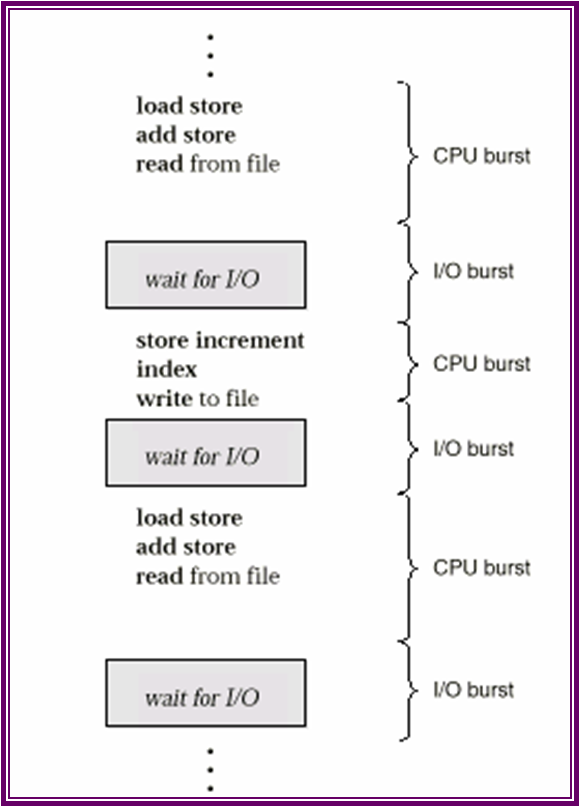
\includegraphics[scale=0.5]{v6f6-1}
    \end{center}
  \end{minipage}
  \end{frame}
  
  %% PAGE
  \begin{frame}
  \frametitle{CPU-I/O burst cycle (2/2)} \pause
  \begin{itemize}
  \item{CPU burst distribution} \pause
  \end{itemize}
  \begin{center}
    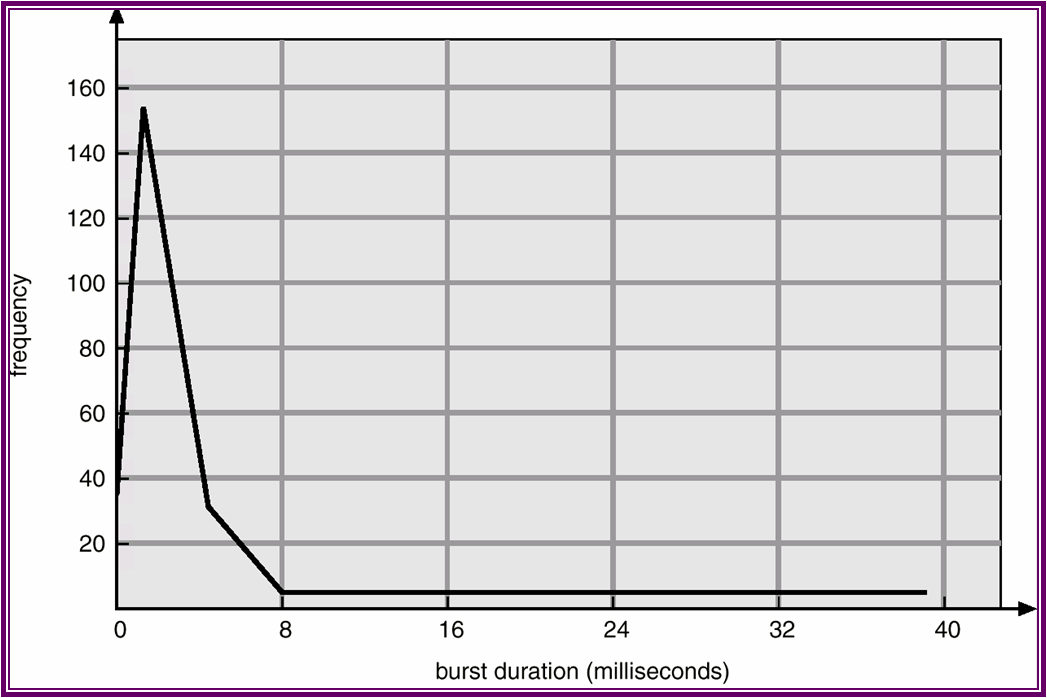
\includegraphics[scale=0.5]{v6f6-2}
  \end{center}
  \end{frame}
  
  \subsection{CPU scheduler}

  %% PAGE
  \begin{frame}
  \frametitle{CPU scheduler} \pause
  \begin{itemize}
  \item{Selects from among the processes in memory that are ready to execute, and allocates the CPU to one of them.} \pause
    \begin{itemize}
    \item{Also known as \textbf{short-term scheduler}.} \pause
    \end{itemize}
  \item{CPU scheduling decisions may take place when a process:} \pause
    \begin{enumerate}
    \item{Switches from running to waiting state.} \pause
    \item{Switches from running to ready state.} \pause
    \item{Switches from waiting to ready.} \pause
    \item{Terminates.} \pause
    \end{enumerate}
  \item{Scheduling under 1 and 4 is \textbf{non-preemptive}. All other scheduling is \textbf{preemptive}.}
  \end{itemize}
  \end{frame}
  
  \subsection{Dispatcher}

  %% PAGE
  \begin{frame}
  \frametitle{Dispatcher} \pause
  \begin{itemize}
  \item{\emph{Dispatcher} module gives control of the CPU to the process selected by the short-term scheduler; this involves:} \pause
    \begin{itemize}
    \item{switching context} \pause
    \item{switching to user mode} \pause
    \item{jumping to the proper location in the user program to restart that program} \pause
    \end{itemize}
  \item{\emph{Dispatch latency} \pause– time it takes for the dispatcher to stop one process and start another running.}
  \end{itemize}
  \end{frame}
  
  \subsection{Scheduling criteria}

  %% PAGE
  \begin{frame}
  \frametitle{Scheduling criteria} \pause
  \begin{itemize}
  \item{CPU utilization \pause –  keep the CPU as busy as possible} \pause
  \item{Throughput \pause –  \# of processes that complete their execution per time unit} \pause
  \item{Turnaround time \pause –  amount of time to execute a particular process} \pause
  \item{Waiting time \pause –  amount of time a process has been waiting in the ready queue} \pause
  \item{Response time \pause –  amount of time it takes from when a request was submitted until the first response is produced}
  \end{itemize}
  \end{frame}
  
  \section{Scheduling algorithms}

  \subsection{First-come, first-served}

  %% PAGE
  \begin{frame}
  \frametitle{First-come, first-served (FCFS)} \pause
  \begin{itemize}
  \item{Example} \pause
  \end{itemize}
  \begin{center}
	\rowcolors[]{1}{blue!20}{blue!10}
    \begin{tabular}{cc}
      Process & Burst time\\
      \hline
      $P_1$ & 24\\
      $P_2$ & 3\\
      $P_3$ & 3
    \end{tabular} \pause
  \end{center}
  \begin{itemize}
  \item{Suppose that the processes arrive in the order: $P_1$, $P_2$, $P_3$. The \emph{Gantt Chart} for the schedule is:} \pause
  \end{itemize}
  \begin{center}
    \setlength{\unitlength}{0.5cm}
    \begin{picture}(20, 2.5)
      \put(-0.2, 0){0}
      \put(0, 1){\framebox(16, 1.5){$P_1$}}
      \put(15.5, 0){24}
      \pause
      \put(16, 1){\framebox(2, 1.5){$P_2$}}
      \put(17.5, 0){27}
      \pause
      \put(18, 1){\framebox(2, 1.5){$P_3$}}
      \put(19.5, 0){30}
      \pause
    \end{picture}
  \end{center}
  \begin{itemize}
  \item{Waiting time for P1  = 0; P2  = 24; P3 = 27} \pause
  \item{Average waiting time:  (0 + 24 + 27)/3 = 17}
  \end{itemize}
  \end{frame}
  
  \subsection{Shortest Job First}

  %% PAGE
  \begin{frame}
  \frametitle{Shortest-Job-First (SJF)} \pause
  \begin{itemize}
  \item{Associate with each process the length of its next CPU burst.} \pause
    \begin{itemize}
    \item{Use these lengths to schedule the process with the shortest time.} \pause
    \end{itemize}
  \item{Two schemes:} \pause
    \begin{itemize}
    \item{Non-preemptive \pause - once CPU given to the process it cannot be preempted until completes its CPU burst.} \pause
    \item{Preemptive \pause - if a new process arrives with CPU burst length less than remaining time of current executing process, preempt.} \pause
      \begin{itemize}
      \item{This scheme is known as the \emph{Shortest-Remaining-Time-First (SRTF)}.} \pause
      \end{itemize}
    \end{itemize}
  \item{SJF is optimal gives minimum average waiting time for a given set of processes.}
  \end{itemize}
  \end{frame}
  
  %% PAGE
  \begin{frame}
  \frametitle{Example: Non-preemptive SJF} \pause
  \begin{center}
	\rowcolors[]{1}{blue!20}{blue!10}
    \begin{tabular}{ccc}
      Process & Arrival time & Burst time\\
      \hline
      $P_1$ & 0 & 7\\
      $P_2$ & 2 & 4\\
      $P_3$ & 4 & 1\\
      $P_4$ & 5 & 4
    \end{tabular} \pause
  \end{center}
  \begin{itemize}
  \item{Non-preemptive SJF} \pause
  \end{itemize}
  \begin{center}
    \setlength{\unitlength}{0.5cm}
    \begin{picture}(20, 2.5)
      \put(-0.2, 0){0}
      \put(0, 1){\framebox(7, 1.5){$P_1$}}
      \put(6.8, 0){7}
      \pause
      \put(7, 1){\framebox(1, 1.5){$P_3$}}
      \put(7.8, 0){8}
      \pause
      \put(8, 1){\framebox(4, 1.5){$P_2$}}
      \put(11.5, 0){12}
      \pause
      \put(12, 1){\framebox(4, 1.5){$P_4$}}
      \put(15.5, 0){16}
      \pause
    \end{picture}
  \end{center}
  \begin{itemize}
  \item{Average waiting time = (0 + 6 + 3 + 7)/4 = 4.} 
  \end{itemize}
  \end{frame}
  
  %% PAGE
  \begin{frame}
  \frametitle{Example: Preemptive SJF} \pause
  \begin{center}
	\rowcolors[]{1}{blue!20}{blue!10}
    \begin{tabular}{ccc}
      Process & Arrival time & Burst time\\
      \hline
      $P_1$ & 0 & 7\\
      $P_2$ & 2 & 4\\
      $P_3$ & 4 & 1\\
      $P_4$ & 5 & 4
    \end{tabular} \pause
  \end{center}
  \begin{itemize}
  \item{Preemptive SJF} \pause
  \end{itemize}
  \begin{center}
    \setlength{\unitlength}{0.5cm}
    \begin{picture}(20, 2.5)
      \put(-0.2, 0){0}
      \put(0, 1){\framebox(2, 1.5){$P_1$}}
      \put(1.8, 0){2}
      \pause
      \put(2, 1){\framebox(2, 1.5){$P_2$}}
      \put(3.8, 0){4}
      \pause
      \put(4, 1){\framebox(1, 1.5){$P_3$}}
      \put(4.8, 0){5}
      \pause
      \put(5, 1){\framebox(2, 1.5){$P_2$}}
      \put(6.8, 0){7}
      \pause
      \put(7, 1){\framebox(4, 1.5){$P_4$}}
      \put(10.5, 0){11}
      \pause
      \put(11, 1){\framebox(5, 1.5){$P_1$}}
      \put(15.5, 0){16}
      \pause
    \end{picture}
  \end{center}
  \begin{itemize}
  \item{Average waiting time = (9 + 1 + 0 + 2)/4 = 3.}
  \end{itemize}
  \end{frame}
  
  \subsection{Priority scheduling}

  %% PAGE
  \begin{frame}
  \frametitle{Priority scheduling} \pause
  \begin{itemize}
  \item{A priority number (integer) is associated with each process} \pause
    \begin{itemize}
    \item{SJF is a priority scheduling where priority is the next CPU burst time.} \pause
    \end{itemize}
  \item{The CPU is allocated to the process with the highest priority.} \pause
    \begin{itemize}
    \item{It can be preemptive or non-preemptive}
    \end{itemize}

  \item{Problems} \pause
    \begin{enumerate}
    \item{\emph{Starvation} \pause - low priority processes may never execute.} \pause
    \item{\emph{Priority inversion} \pause - higher-priority process need to access a resource being held by another lower-priority process.} \pause
    \end{enumerate}
  \item{Solution} \pause
    \begin{itemize}
    \item{\emph{Aging} \pause - increasing the priority of the process with
      time going on.}
    \end{itemize}
  \end{itemize}
  \end{frame}
  
  \subsection{Round-Robin scheduling}

  %% PAGE
  \begin{frame}
  \frametitle{Round-Robin scheduling (RR)} \pause
  \begin{itemize}
  \item{Each process gets a small unit of CPU time (time \emph{quantum} or \emph{slice}), usually 10-100 milliseconds.} \pause
    \begin{itemize}
    \item{After this time has elapsed, the process is preempted and added to the end of the ready queue.} \pause
    \end{itemize}
  \item{If there are \textit{n} processes in the ready queue and the time quantum is \textit{q},} \pause
    \begin{itemize}
    \item{then each process gets \textit{1/n} of the CPU time in chunks of at most \textit{q} time units at once.} \pause
    \item{No process waits more than \textit{(n-1)q} time units.} \pause
    \end{itemize}
  \item{Performance} \pause
    \begin{itemize}
    \item{\textit{q} large \pause - FCFS} \pause
    \item{\textit{q} small \pause - \textit{q} must be large with respect to context switch, otherwise overhead is too high.}
    \end{itemize}
  \end{itemize}
  \end{frame}
  
  \subsection{Multilevel queue}

  %% PAGE
  \begin{frame}
  \frametitle{Multilevel queue (1/2)} \pause
  \begin{itemize}
  \item{Ready queue is further partitioned into separate queues:} \pause
    \begin{itemize}
    \item{A priority number is associated with each queue.} \pause
    \item{Example: foreground (for interactive processes) and background (for batch processes) queues.} \pause
    \end{itemize}
  \item{Each queue has its own scheduling algorithm,} \pause
    \begin{itemize}
    \item{foreground uses RR; background uses FCFS, for example.} \pause
    \end{itemize}
%  \item{Scheduling must be done between the queues.} \pause
%    \begin{itemize}
%    \item{Fixed priority scheduling: \pause serve all from foreground then from background.} \pause
%      \begin{itemize}
%      \item{Possibility of starvation.} \pause
%      \end{itemize}
%    \item{Time slice: \pause each queue gets a certain amount of CPU time which it can schedule amongst its processes. For example, 80\% to foreground in RR, 20\% to background in FCFS.}
%    \end{itemize}
  \end{itemize}
  \end{frame}
  
  %% PAGE
  \begin{frame}
  \frametitle{Multilevel queue (2/2)} \pause
  \begin{center}
    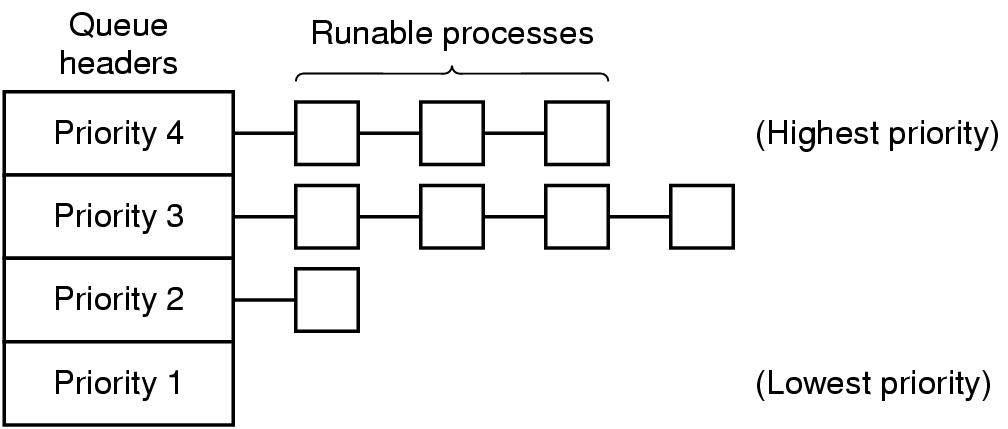
\includegraphics[scale=0.35]{mosv2f2-42}
  \end{center}
  \end{frame}
  
  \subsection{Multilevel feedback queue}

  %% PAGE
  \begin{frame}
  \frametitle{Multilevel feedback queue scheduling} \pause
  \begin{center}
    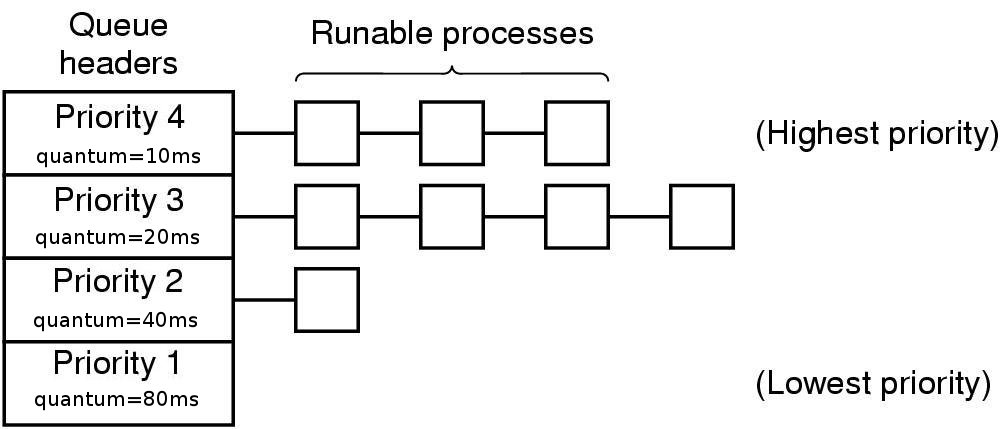
\includegraphics[scale=0.4]{mlfbq} \pause
  \end{center}
  \begin{itemize}
  \item{A process can move between the various queues.} \pause
    \begin{itemize}
    \item{For example, whenever a process used up the quantum allocated to it, it sank into a lower priority queue.}
    \end{itemize}
  \end{itemize}
  \end{frame}
  
  \subsection{Conclusion}

  %% PAGE
  \begin{frame}
  \frametitle{Conclusion} \pause
  \begin{itemize}
  \item{\emph{Getting it right in practice is much harder than getting it right in principle}.} \pause
    \begin{itemize}
    \item{As a result, the scheduler rarely makes the best choice.} \pause
    \item{The solution: \pause separation of scheduling policy and scheduling mechanism.} \pause
      \begin{itemize}
      \item{That is, the scheduling algorithm is parameterized in some way, but the parameters can be filled in by the user.}
      \end{itemize}
    \end{itemize}
  \end{itemize}
  \end{frame}
  
  %% PAGE
  \begin{frame}
  \frametitle{Questions}
  \begin{itemize}
  \item{Any questions?}
  \end{itemize}
  \begin{center}
    
\includegraphics[scale=.5]{question}
  \end{center}
  \end{frame}
  
  %% PAGE
\end{CJK*}
\end{document}
